\documentclass[a4paper]{article}


\usepackage{stmaryrd}

\usepackage{amsmath,amsfonts,amssymb, commath,fancyhdr,mathtools,bm,dsfont,relsize}
\usepackage[margin= 1.0 in]{geometry}
\usepackage[utf8]{inputenc}
\usepackage{amsthm,graphicx,xifthen,dsfont}
\usepackage[linesnumbered, noend, noline]{algorithm2e} %to write algos
\usepackage{multicol} %package for columns
\usepackage{mdframed} %for framed boxes
\usepackage{pgfplots} % graphs in doc
\usepackage{ragged2e} %for alignment of text
\usepackage{lipsum} %random text
\usepackage{wasysym}
\usepackage{enumerate}
\usepackage{cancel}
\usepackage{float}
\usepackage{marginnote} %package for notes in margins
\usepackage{romannum} %Roman numerals
\usepackage{authblk} %Author stuff

\allowdisplaybreaks

\usepackage[square, numbers, sort]{natbib} %Bibliography stuff
\bibliographystyle{abbrvnat}

\usepackage{mathpazo}

%Paragraph and Page formatting commands
\renewcommand{\baselinestretch}{1.15}
\setlength{\parindent}{0em}
\setlength{\parskip}{1em}

\newcommand{\R}{\mathbb{R}}
\newcommand{\Wc}{\mathcal{W}}


\title{\vspace{-2em} 15780 Project: Speeding Up Convolutional Neural Networks with Tensor Decompositions}
\author{Graham Gobieski \quad  Shouvik Mani \quad  Aditya Krishnan}
\date{ \vspace{-2em}}
\begin{document}
\maketitle

CNNs have revolutionized machine learning and AI techniques to solve problems in computer vision. A fundamental component of CNNs are convolution tensors, used to simplify the inputs to the layer by extracting important features of the input. In recent years there has been significant interest in speeding up CNNs by finding good approximations for the convolutional kernels, for example, there has been some work trying to approximate the kernels with low-rank approximations and clustering schemes. Our objective in the project was to find decompositions schemes for tensors that can be used to decompose the convolution kernels thereby, hopefully, dramatically reducing the number of variables that need to be trained. 

We specifically focus on the Tucker-decomposition of tensors. For a 3D-tensor $\mathcal{X} \in \R^{I \times J \times K}$, tucker decomposition of $\mathcal{X}$ denoted by $\llbracket \mathcal{G}; A, B, C \rrbracket$ is an extension of $\mathsf{SVD}$ for higher dimensions. The decomposition is given by three matrices, $A \in \R^{I \times R}$, $B \in \R^{J \times S}$, $C \in \R^{K \times T}$ and a core tensor $\mathcal{G} \in \R^{R \times S \times T}$ such that: 
$$ \sum_{r, s , t} g_{rst} \cdot \vec{a}_r \circ \vec{b}_s \circ \vec{c}_t  $$
where $\circ$ corresponds to the outer product of vectors in higher dimensions and $\vec{a}, \vec{b}, \vec{c}$ are column vectors in $A, B, C$ respectively. A visualization of the decomposition is given below: 
\begin{center}
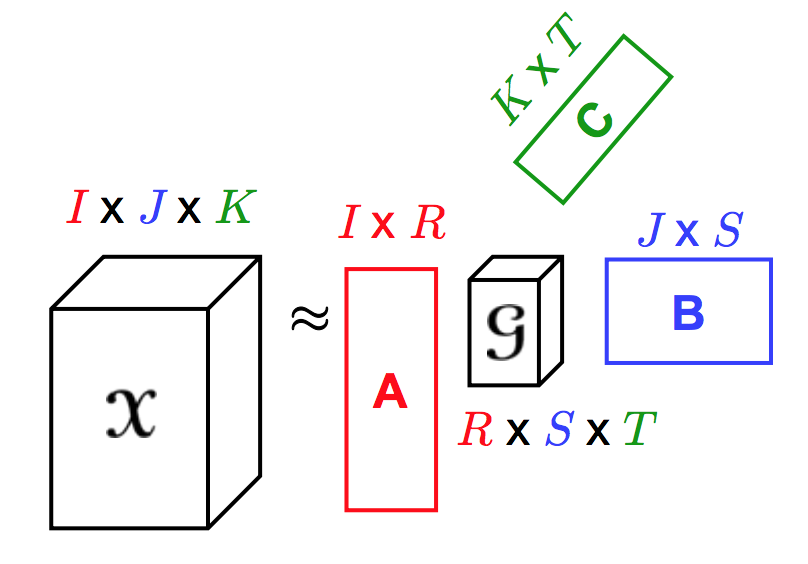
\includegraphics[scale=0.3]{tucker}
\end{center}

A convolutional kernel in a CNN is a 4D-tensor $\Wc \in \R^{N \times d \times d \times C}$, where $N, C$ are the numbers of the output and input features respectively and $d$ is the spatial kernel size. Since $d$ is generally small, we hypothesize that the benefit of the decomposition is in discovering the relationship between the input features, output features and spatial dimension. Hence, we imagine the spatial dimensions to be flattened into vectors in $\R^{d^2}$. 

Our objective then is to find approximations of $\Wc$ by building a decomposition $\llbracket \mathcal{G}; W_N, W_C, W_D\rrbracket$ such that $W_N \in \R^{N \times N'}$, $W_C \in \R^{C \times C'}$, $W_D \in \R^{d^2 \times D'}$ and  the core $\mathcal{G} \in \R^{N' \times C' \times D'}$. Here, $N', C', D'$ are hyper-parameters that will need to be trained.

For the input matrix $Z \in \R^{X \times Y \times C}$, we would compute 
$$W \star Z = \sum_{n', c', d'} \left( g_{n'c'd'} \cdot (\vec{w}_n)_{n'} \circ (\vec{w}_c)_{c'} \circ (\vec{w}_d)_{d'} \star Z \right)$$ 
The runtime of computing a standard convolution $W \star Z$ would be approximately $O(NXYCd^2)$ while computing this convolution is a $O(N'C'D')$ factor greater. Even though computing the convolution is greater, the number of parameters is $O(N'C'D' + NN' + CC' + d^2D')$ as compared to $NCd^2$ paramters that need training without the decomposition. Our hypothesis is that for small values of $N',C',D'$ we can get a significant speedup in the convergence rate of training the parameters of the CNN. 

The Tucker-decomposition is a high dimension generalization of \textsf{SVD}, our motivation for using decomposing the convolutional networks is to capture the relationships between the different dimensions of the tensor and in doing so reduce the number of redundant dimensions. The matrix $W_N$ captures how the output parameters relate to each other and similarly $W_C$ and $W_D$ capture how the input parameters relate to each other and the spatial parameters relate to each other respectively. The core $\mathcal{G}$ captures how the groups relate to one and other. Hence, in practical applications where the parameters have small subspaces that determine them, the decomposition can drastically reduce the number of parameters.

It is not completely clear yet how to perform back-propagation on this decomposition. We make an attempt at trying to give the back-prop gradients with respect to the parameters of the decomposition. Let $\tilde{W}(\mathcal{G}, W_N, W_C, W_D) = \llbracket \mathcal{G}; W_N, W_C, W_D \rrbracket$ be the convolution whose Tucker composition we learn. The regular back-propagation algorithm computes the gradient $\frac{\partial l(x, y)}{\partial W}$ but we need to compute $\frac{\partial l(x, y)}{\partial W_N}$, $\frac{\partial l(x, y)}{\partial W_C}$, $\frac{\partial l(x, y)}{\partial W_D}$ and $\frac{\partial l(x, y)}{\partial \mathcal{G}}$. Using the chain rule we get that: 
$$\frac{\partial l(x, y)}{\partial X} = \frac{\partial l(x, y)}{\partial \tilde{W}} \cdot \frac{\partial \tilde{W}}{\partial X} $$ 
where $X \in \{\mathcal{G}, W_N, W_C, W_D\}$. Hence, it is sufficient to give the gradients $\frac{\partial \tilde{W}}{\partial X}$ which can then be plugged into the regular back-propagation algorithm for CNNs. 

In order to compute gradients we first give some useful notation. Define $\mathds{1}_{n \times m} \in \R^{n \times m}$ to be a matrix of $1$s. Let $\mathsf{vec}(\mathcal{X})$ be a vector in $\R^{I\cdot J \cdot K}$ for a 3D-tensor $\mathcal{X} \in \R^{I \times J \times K}$ such that $\mathcal{X}_{ijk} = \mathsf{vec}(\mathcal{X})_{i \cdot I + j \cdot J + k}$. Given the tensor $\tilde{W}$, we can write $\mathsf{vec}{\tilde{W}}$ as 
$$\mathsf{vec}(\tilde{W}) = (W_D \otimes W_C \otimes W_N)\mathsf{vec}(\mathcal{G}) $$ 
We now give the gradients of $\mathsf{vec}(\tilde{W})$ with respect to the parameters $W_N, W_D, W_C, \mathcal{G}$
\begin{align*}
&\frac{\partial \mathsf{vec}(\tilde{W})}{\partial W_D} = (\mathds{1}_{d^2 \times D'} \otimes W_C \otimes W_N)\mathsf{vec}(\mathcal{G})
&&\frac{\partial \mathsf{vec}(\tilde{W})}{\partial W_C} = (W_D \otimes \mathds{1}_{C \times C'} \otimes W_N)\mathsf{vec}(\mathcal{G}) \\ 
&\frac{\partial \mathsf{vec}(\tilde{W})}{\partial W_N} = (W_D \otimes W_C \otimes \mathds{1}_{N \times N'})\mathsf{vec}(\mathcal{G})
&&\frac{\partial \mathsf{vec}(\tilde{W})}{\partial \mathcal{G}} = (W_D \otimes W_C \otimes W_N) \cdot \mathds{1}_{C'\cdot D' \cdot N'}
\end{align*}
Where $\mathds{1}_{C'\cdot D' \cdot N'} \in \R^{C'\cdot D' \cdot N'}$ is a vector of $1$s. We tried to show that the gradient under vectorization doesn't change but this doesn't seem to be simple.   

Now that we have explored the changes to back-propagation, we have left to explore the training of the hyper-parameters $N',C',D'$. In order to do so, we suggest computing the full tensor $\tilde{W}$ as we would using the validation data set and then compute the Tucker-decomposition using Higher-Order Orthogonal Iteration. This will give us a candidate $W_N', W_C'$ and $W_D'$. We can then perform \textsf{SVD} on these matrices which would output some singular values $\sigma_1, \dots, \sigma_{i_m}$. By comparing the the relative sizes of the singular values, one can find a integer $k_i \leq i_m$ such that the top $k_i$ singular values are a good low-rank approximation of the matrix. The value $k_i$ for each $i \in \{N, C, D\}$  would then be the values of the hyper-parameters.  





\end{document}